\documentclass[11pt,a4paper]{article}
\usepackage[utf8]{inputenc}
\usepackage[T1]{fontenc}
\usepackage[french]{babel}
\usepackage{geometry}
\usepackage{graphicx}
\usepackage{hyperref}
\usepackage{float}
\usepackage{amsmath}
\usepackage{amssymb}

\geometry{hmargin=2.5cm,vmargin=2.5cm}


\providecommand{\tightlist}{
  \setlength{\itemsep}{0pt}\setlength{\parskip}{0pt}}

\begin{document}


\begin{titlepage}
    \centering
    {\scshape\LARGE Université de Mons \par}
    \vspace{1cm}
    {\scshape\Large Faculté des Sciences -- Sciences Informatiques\par}
    \vspace{1.5cm}
    {\huge\bfseries Projet de Génie Logiciel (S-INFO-015)\par}
    \vspace{0.5cm}
    {\Large\bfseries Rapport du Jalon 1A\par}
    \vspace{1.5cm}
    
    \textbf{Année académique :} 2026-2027\par
    \textbf{Groupe :} G02\par
    \vspace{1cm}

    \begin{tabular}{ll}
        \textbf{Étudiant 1 :} & Berkani Zinediné (Matricule : ) \\
        & \textit{Extension choisie :} Paiement et gestion de fraudes \\[0.2cm]
        \textbf{Étudiant 2 :} & Fontaine Alexis (Matricule : ) \\
        & \textit{Extension choisie :} Gestion de cartes \\[0.2cm]
        \textbf{Étudiant 3 :} & Quarta Hugo (Matricule : 250711) \\
        & \textit{Extension choisie :} Gestion du budget financier \\[0.2cm]
        \textbf{Étudiant 4 :} & Vandooren Romain (Matricule : ) \\
        & \textit{Extension choisie :} Gestion des placements \\
    \end{tabular}

\end{titlepage}

\newpage
\tableofcontents
\newpage


\section{Fonctionnalités de base}

\subsection{Diagrammes de cas d'utilisation (UML)}
\begin{figure}[H]
    \centering
    \makebox[\textwidth][c]{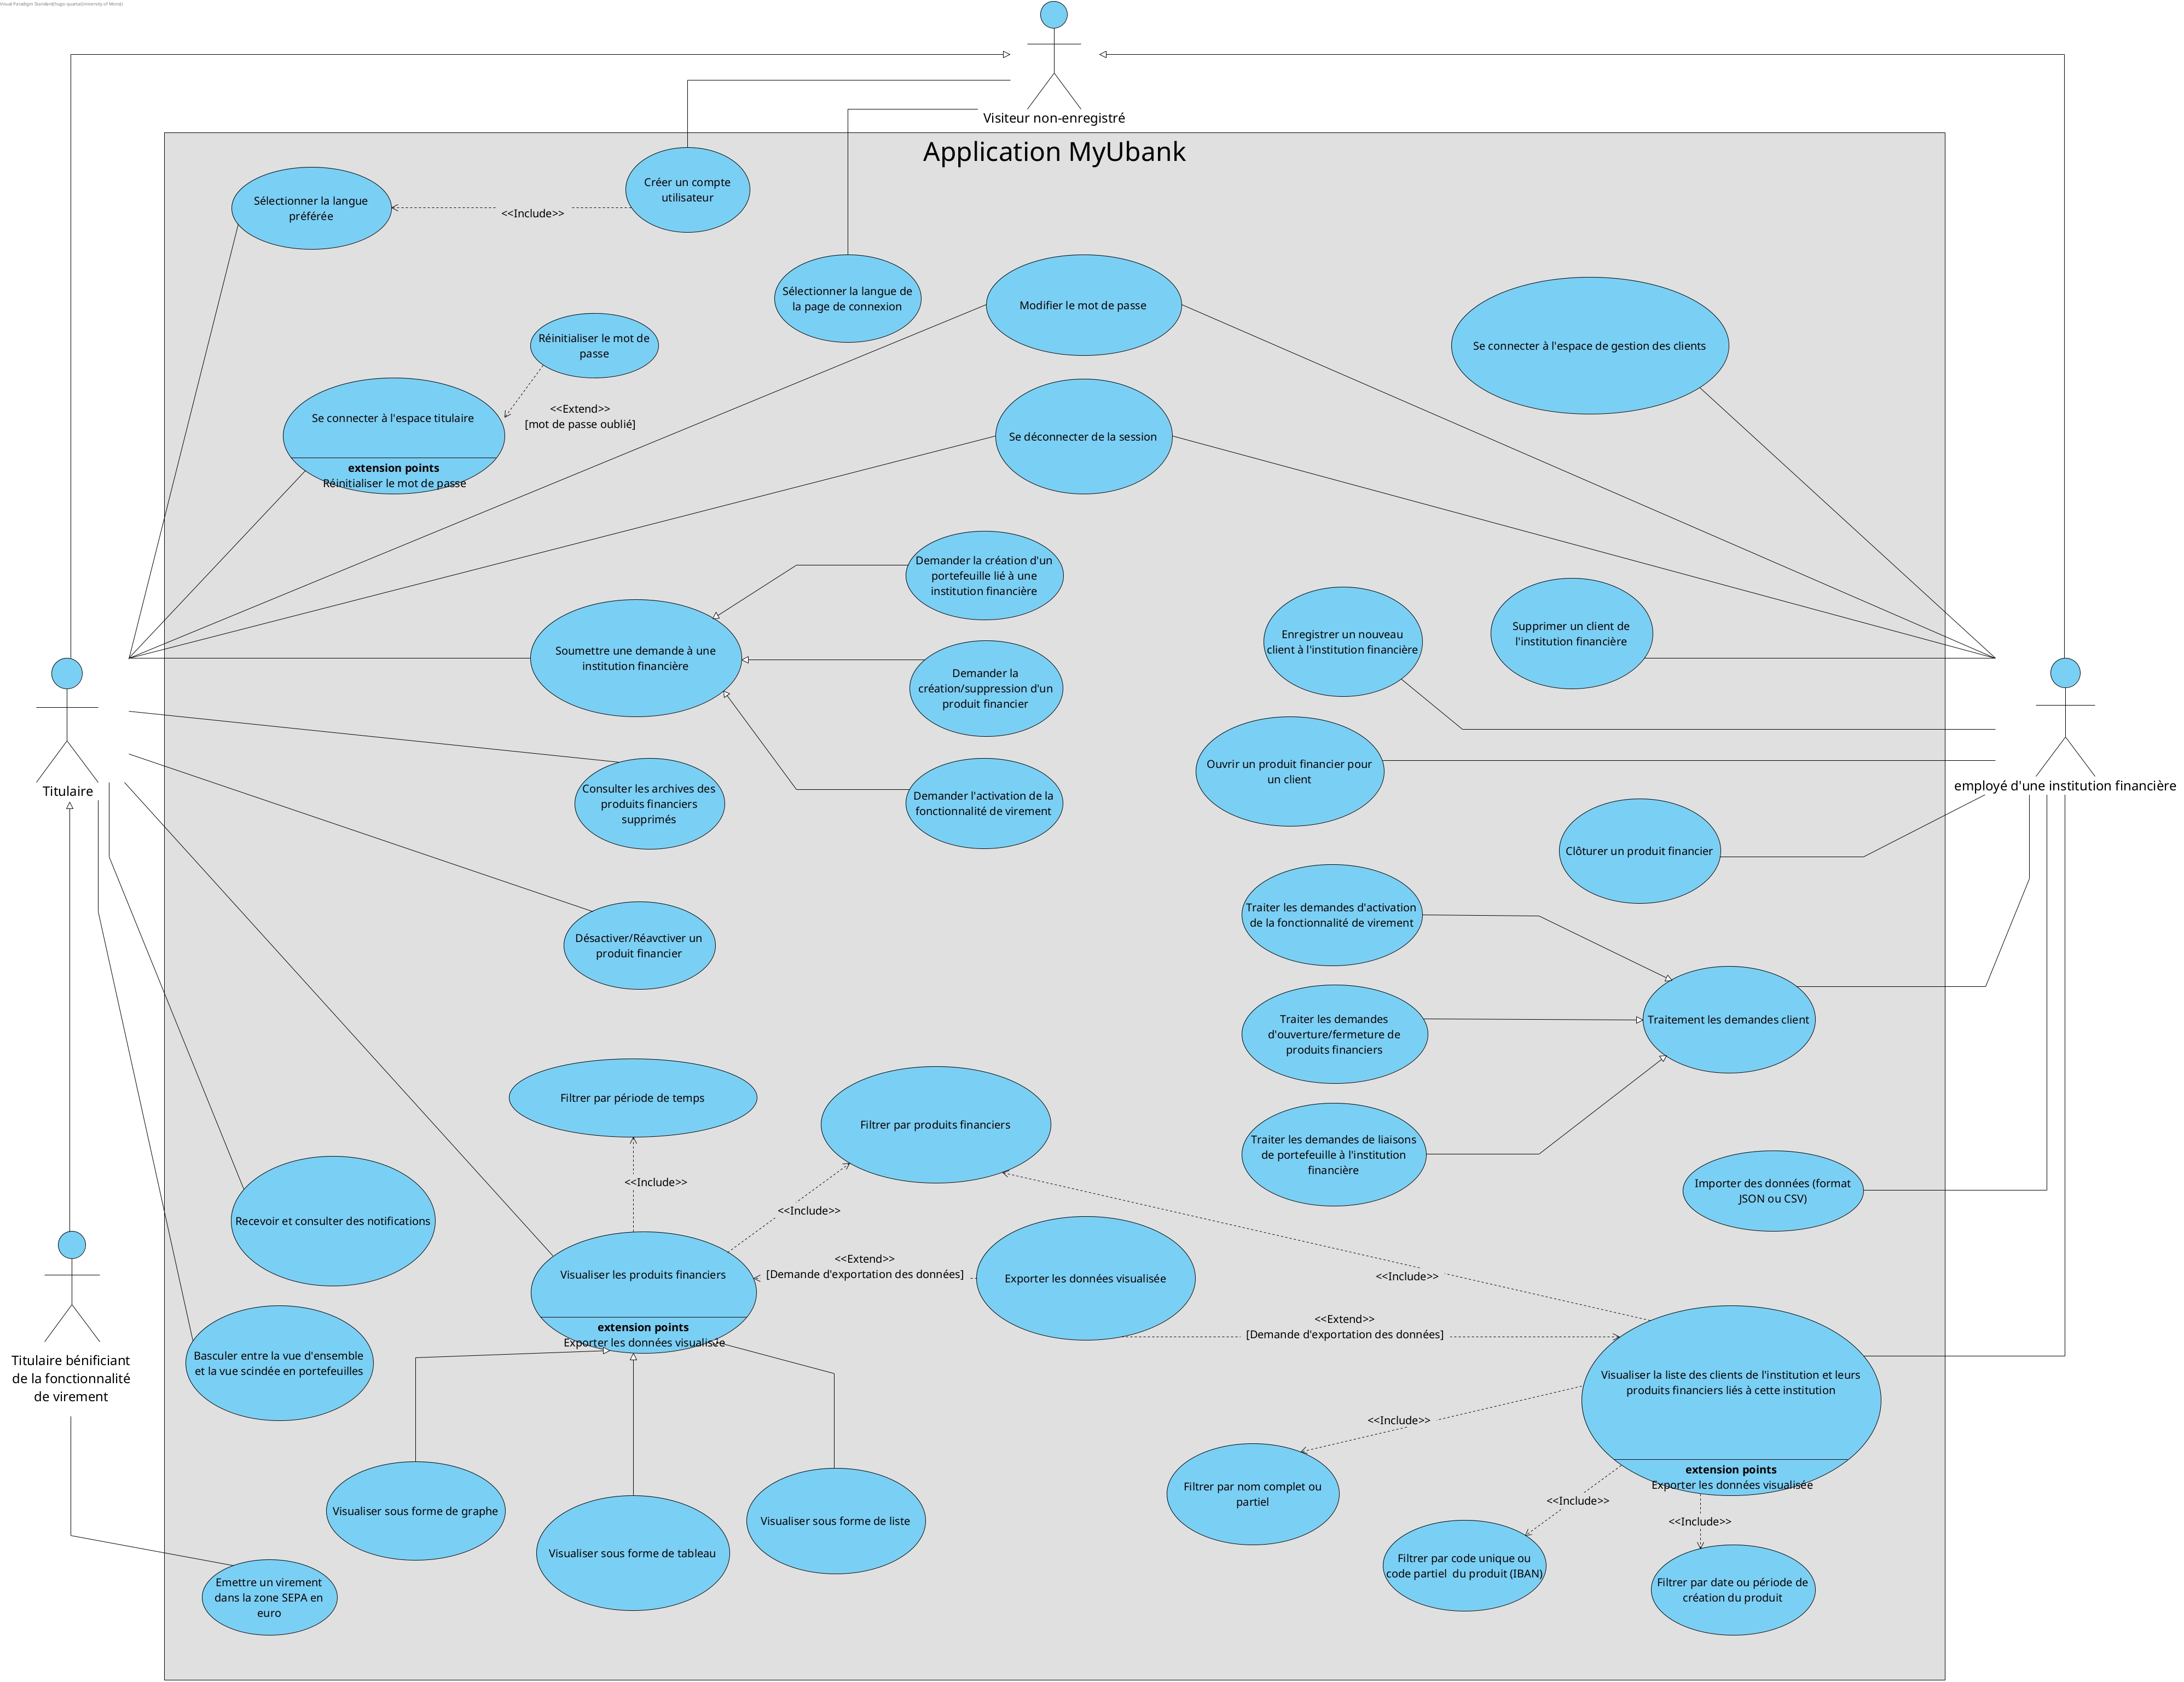
\includegraphics[width=1.3\textwidth]{MyUbankUC.jpg}}
    \caption{Diagramme de cas d'utilisation -- Fonctionnalités de base}
    \label{fig_uc_base}
\end{figure}
\noindent \textit{Le diagramme ci-dessus se trouve dans le projet Visual Paradigme Projet Génie Logiciel G02.vpp et l'image peut être retrouvée dans le fihier "MyUbankUC.jpg" dans l'archive contenant ce rapport.}

\subsection{Interaction Overview Diagram}
\begin{figure}[H]
    \centering
    \makebox[\textwidth][c]{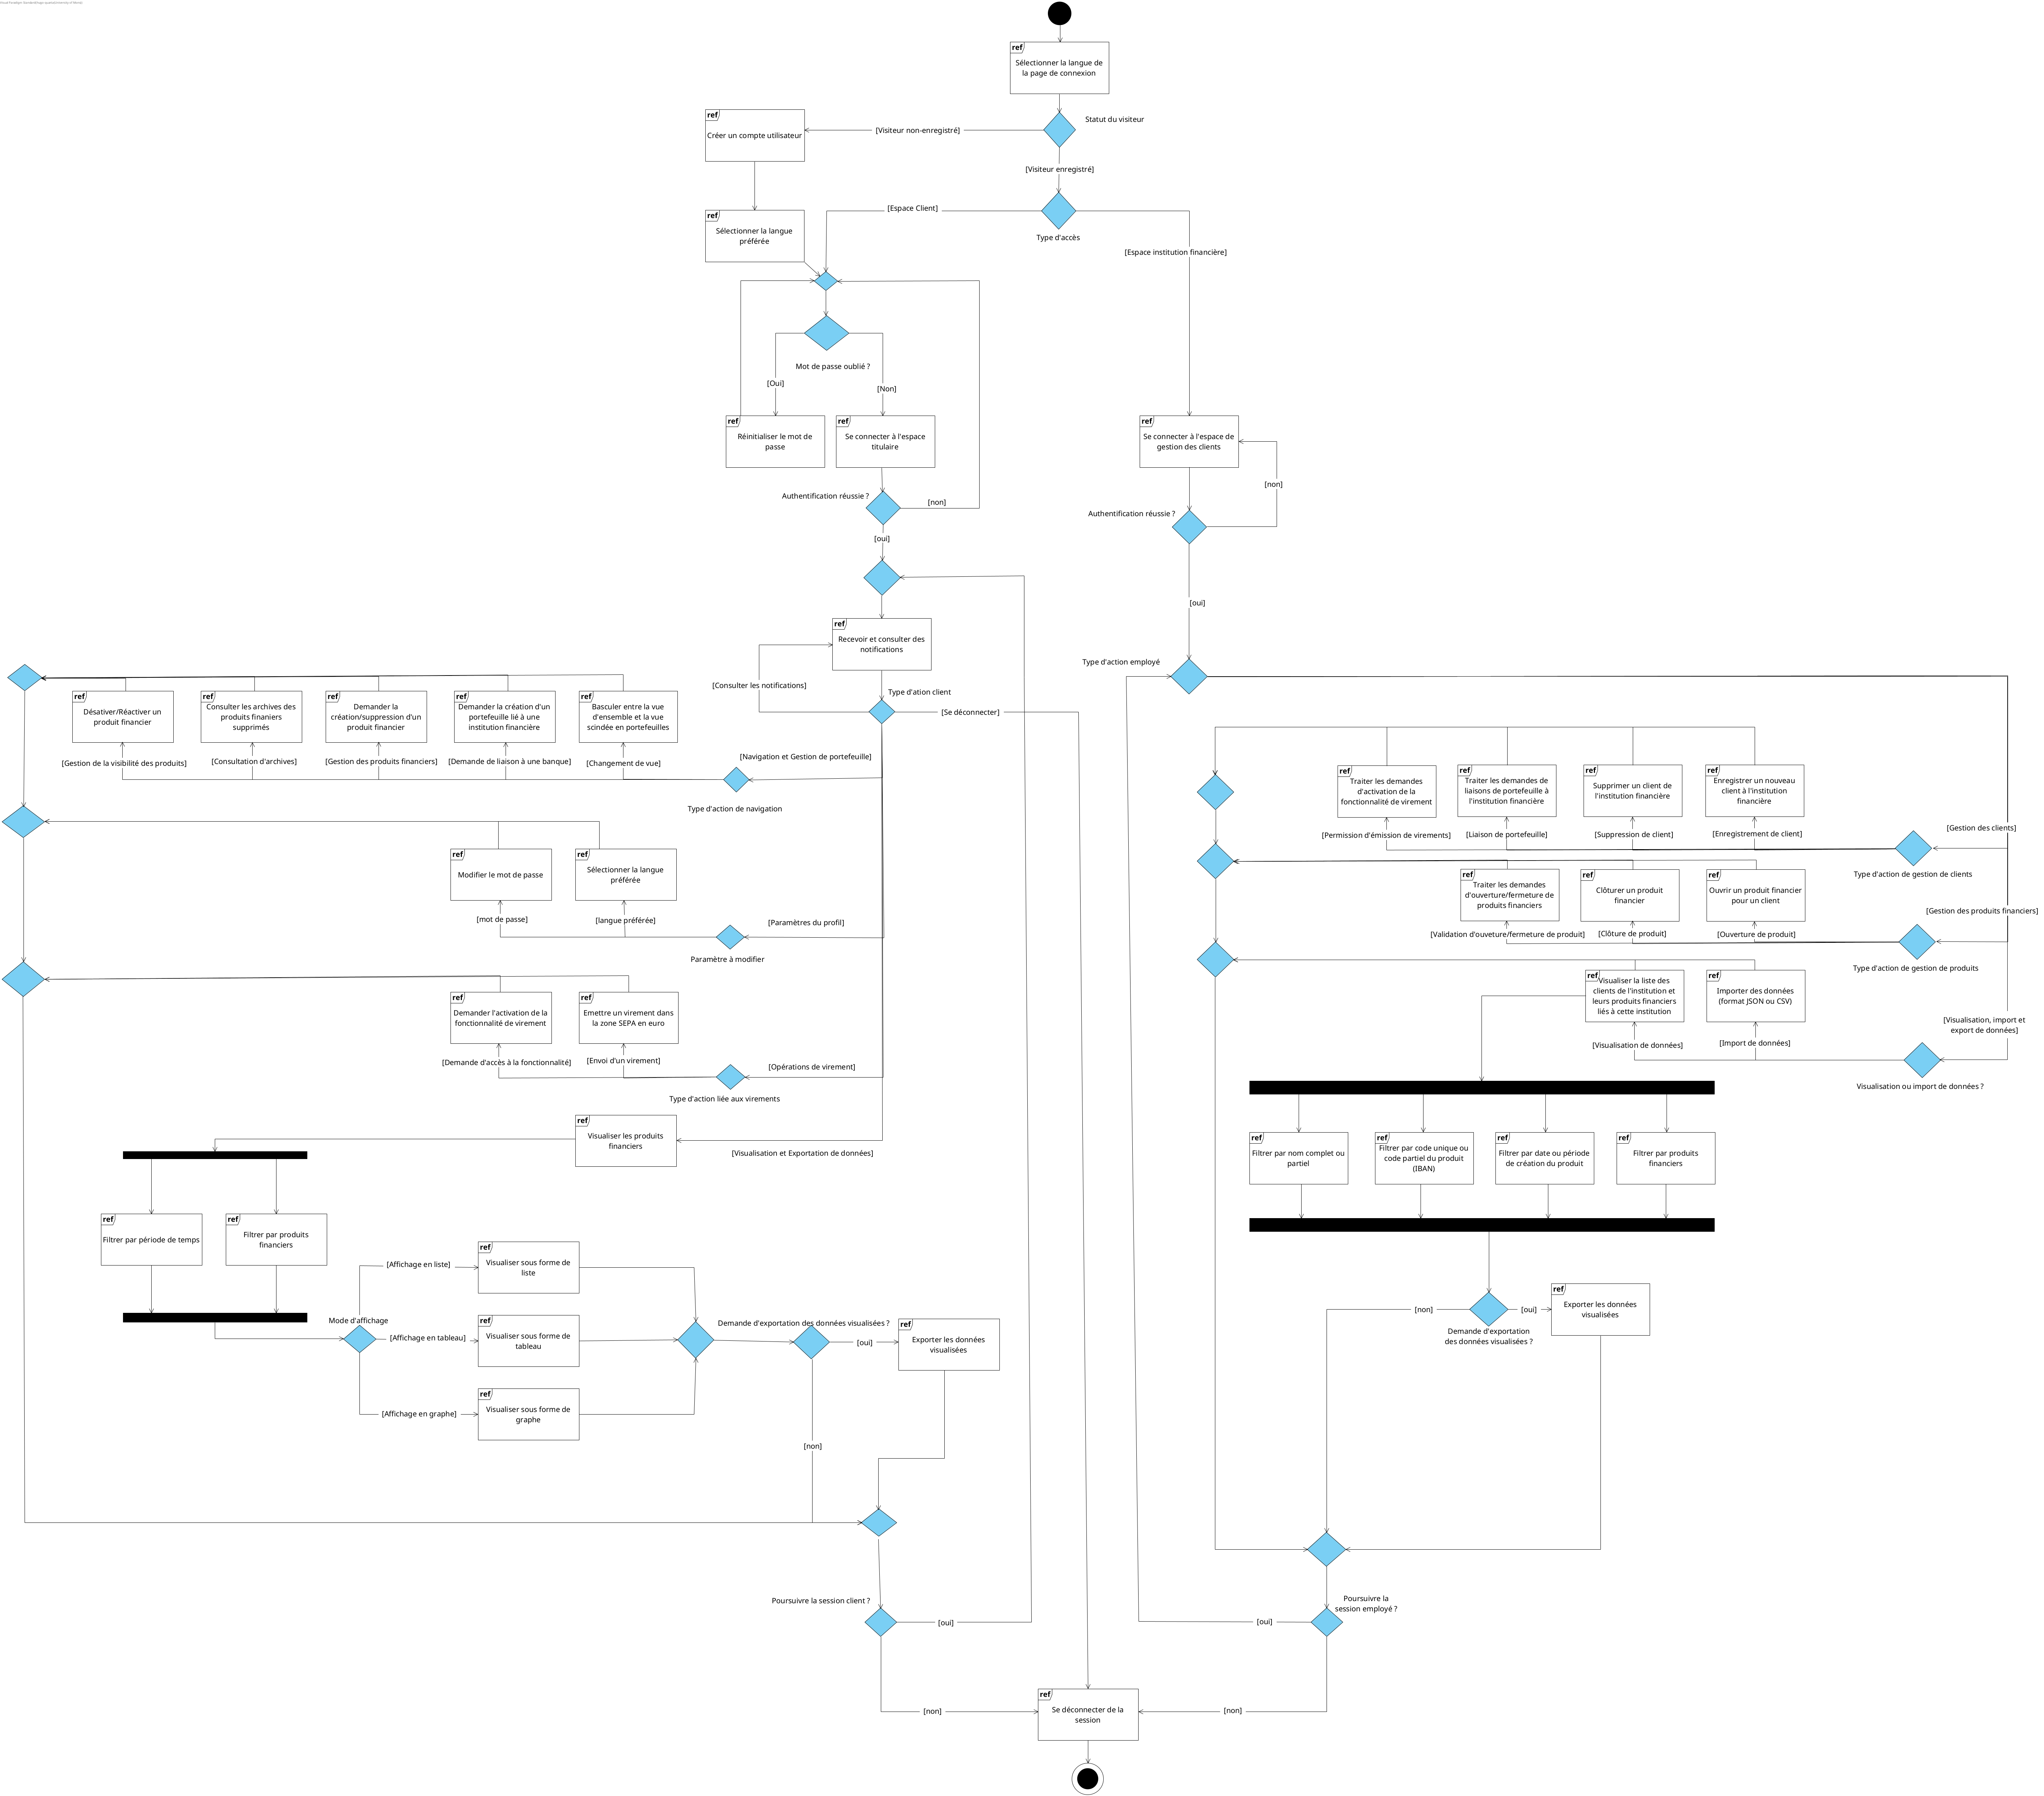
\includegraphics[width=1.3\textwidth]{MyUbankIOD.jpg}}
    \caption{Interaction Overview Diagram -- Fonctionnalités de base}
    \label{fig_iod_base}
\end{figure}
\noindent \textit{Le diagramme ci-dessus se trouve dans le projet Visual Paradigme Projet Génie Logiciel G02.vpp et l'image peut être retrouvée dans le fihier "MyUbankIOD.jpg" dans l'archive contenant ce rapport.}

\pagebreak
Afin de rendre ce diagramme plus lisible, voici un découpage des différentes parties de celui-ci :
\begin{figure}[H]
    \centering
    \makebox[\textwidth][c]{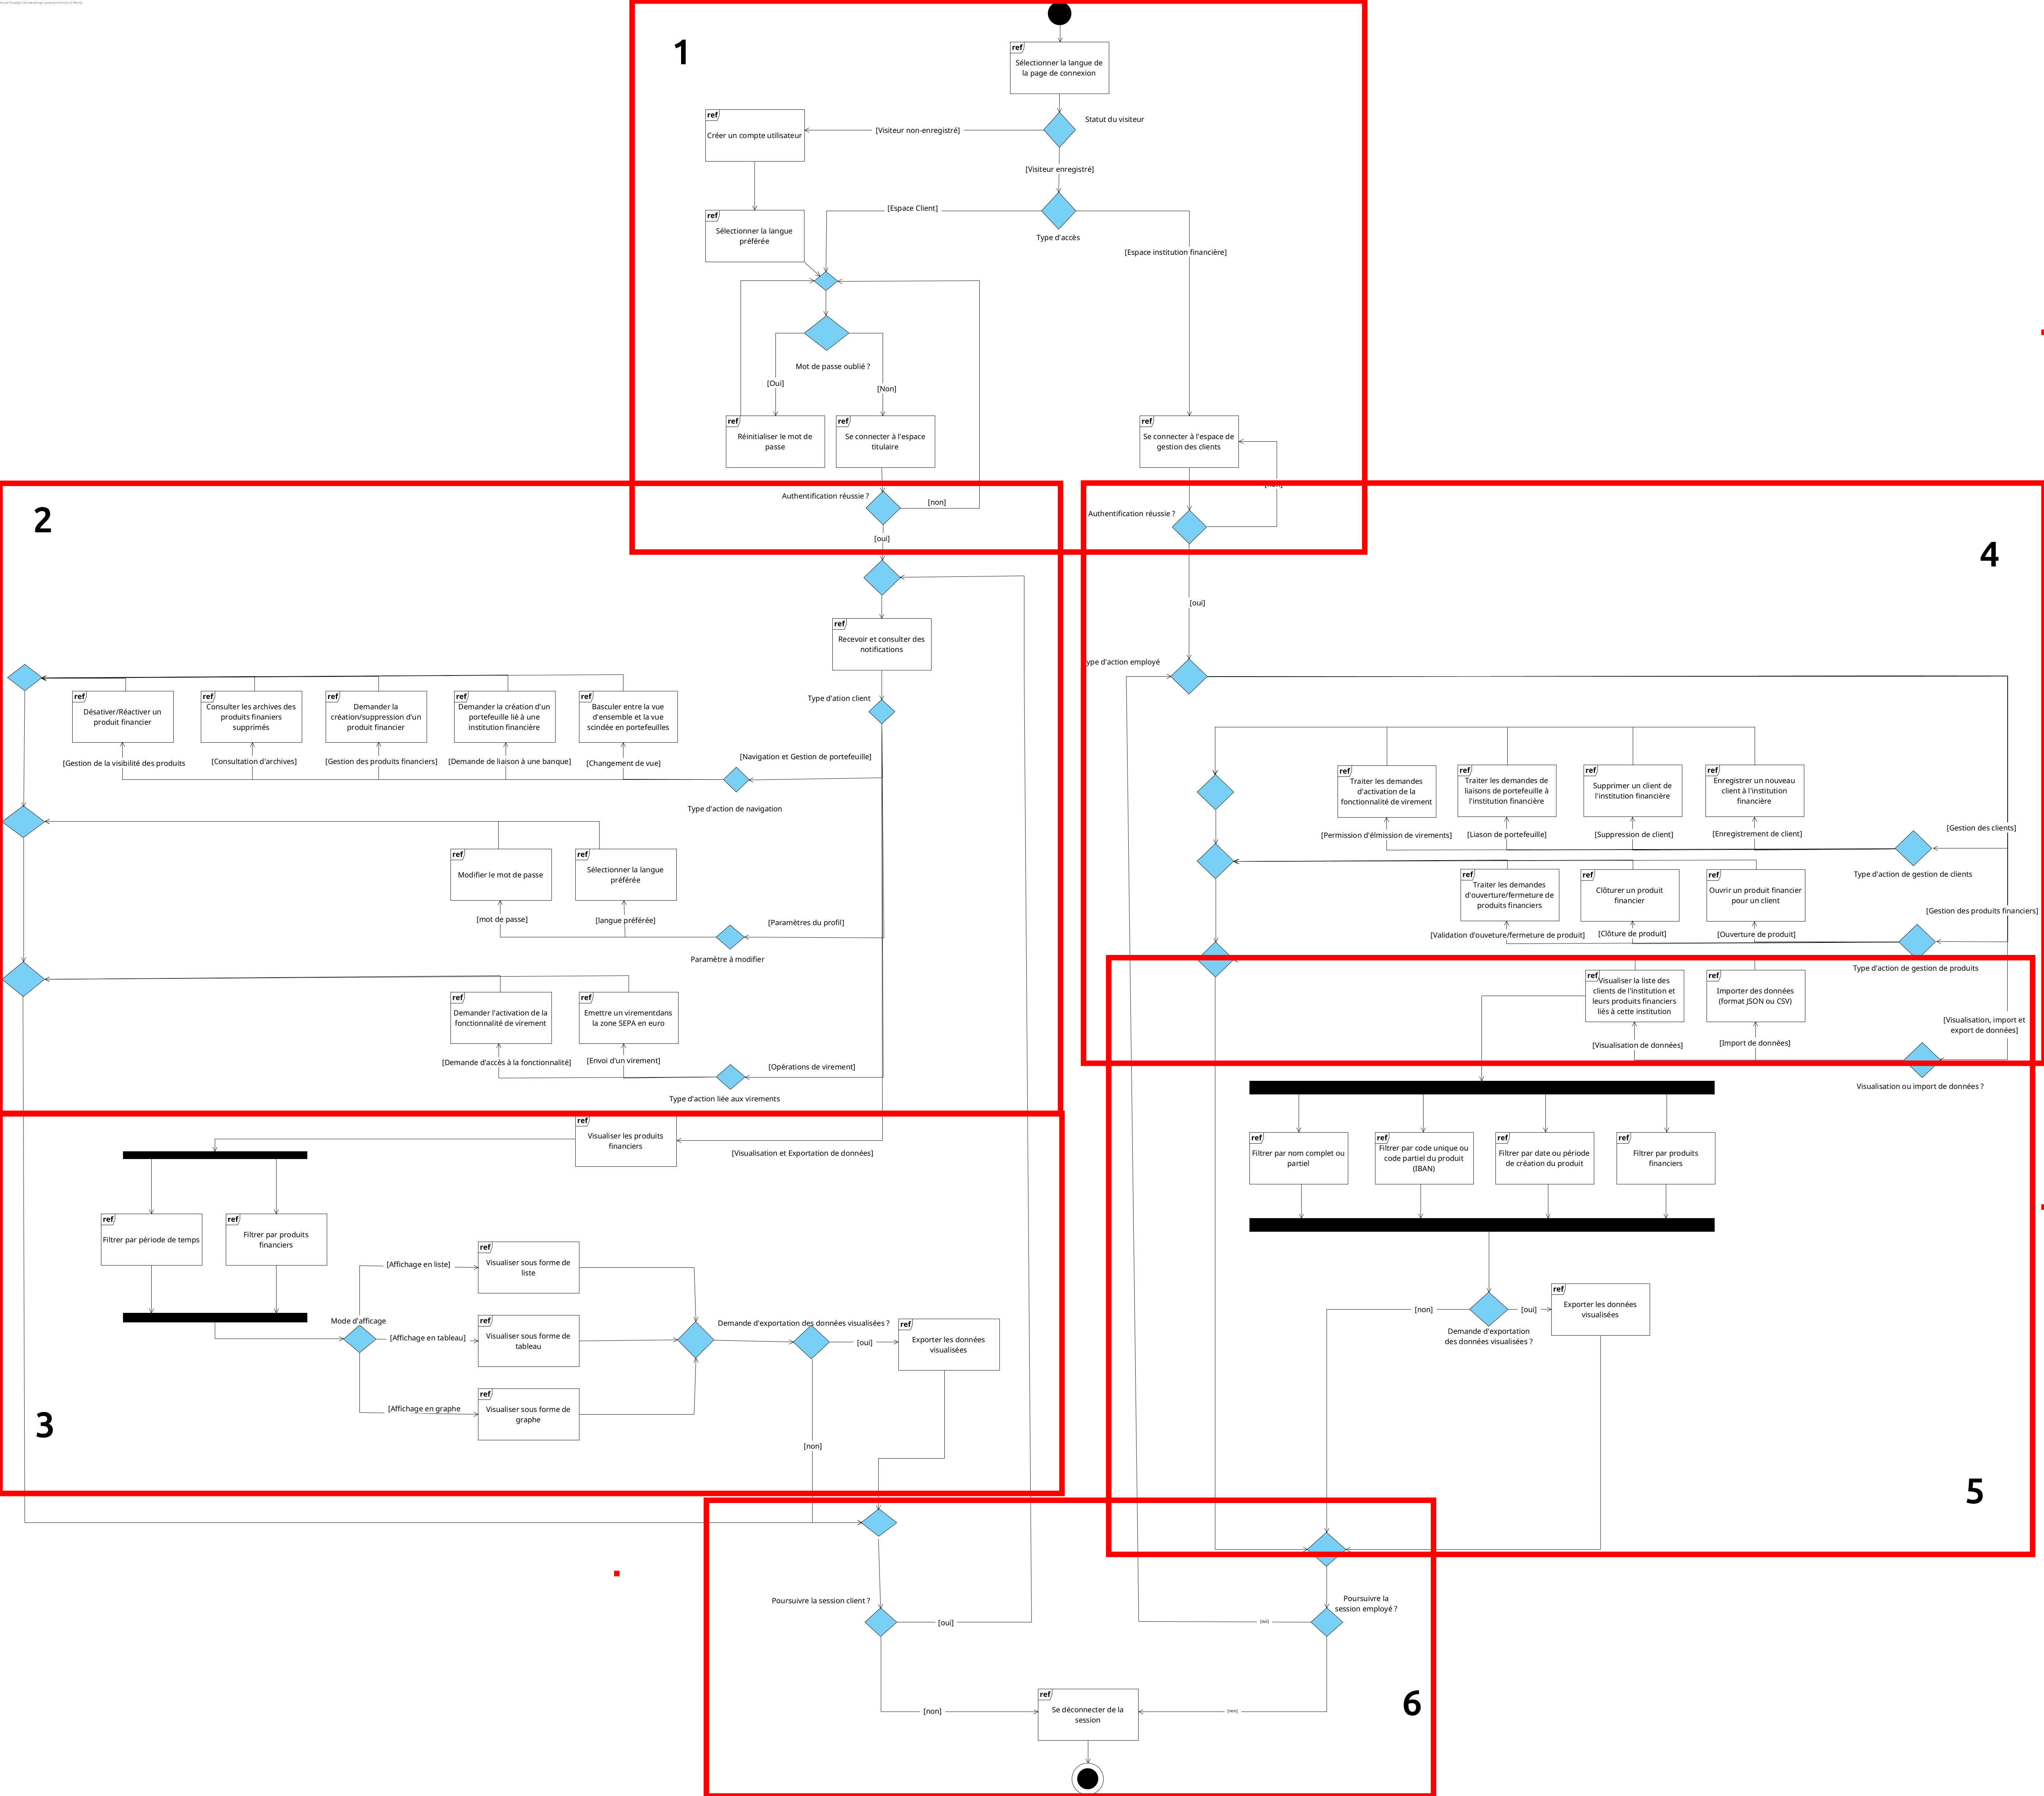
\includegraphics[width=1.3\textwidth]{IOD-Areas/MyUbankIOD-Areas.jpg}}
    \caption{Interaction Overview Diagram -- Découpage}
    \label{fig_iod_areas}
\end{figure}


\subsubsection{IOD - Phase de connexion}
\begin{figure}[H]
    \centering
    \makebox[\textwidth][c]{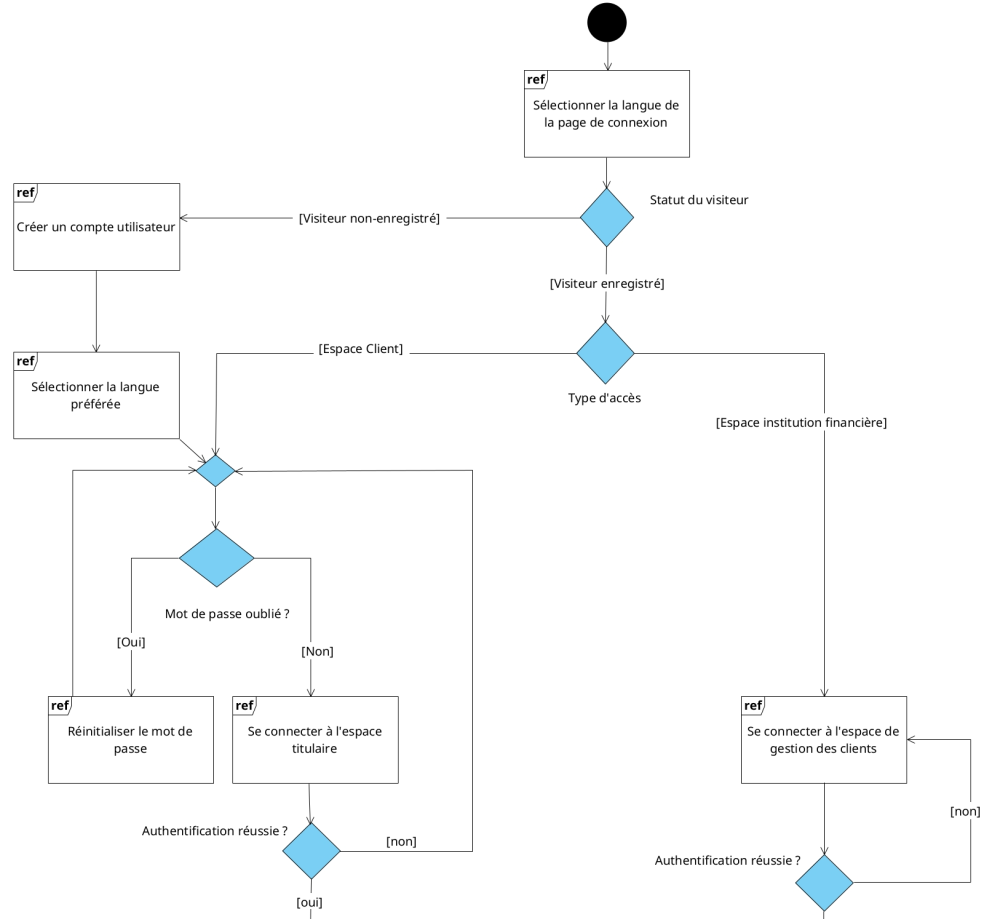
\includegraphics[width=1.0\textwidth]{IOD-Areas/ConnexionArea.png}}
    \caption{Interaction Overview Diagram -- Phase de connexion}
    \label{fig_iod_connexion}
\end{figure}


\subsubsection{IOD - Actions client}
\begin{figure}[H]
    \centering
    \makebox[\textwidth][c]{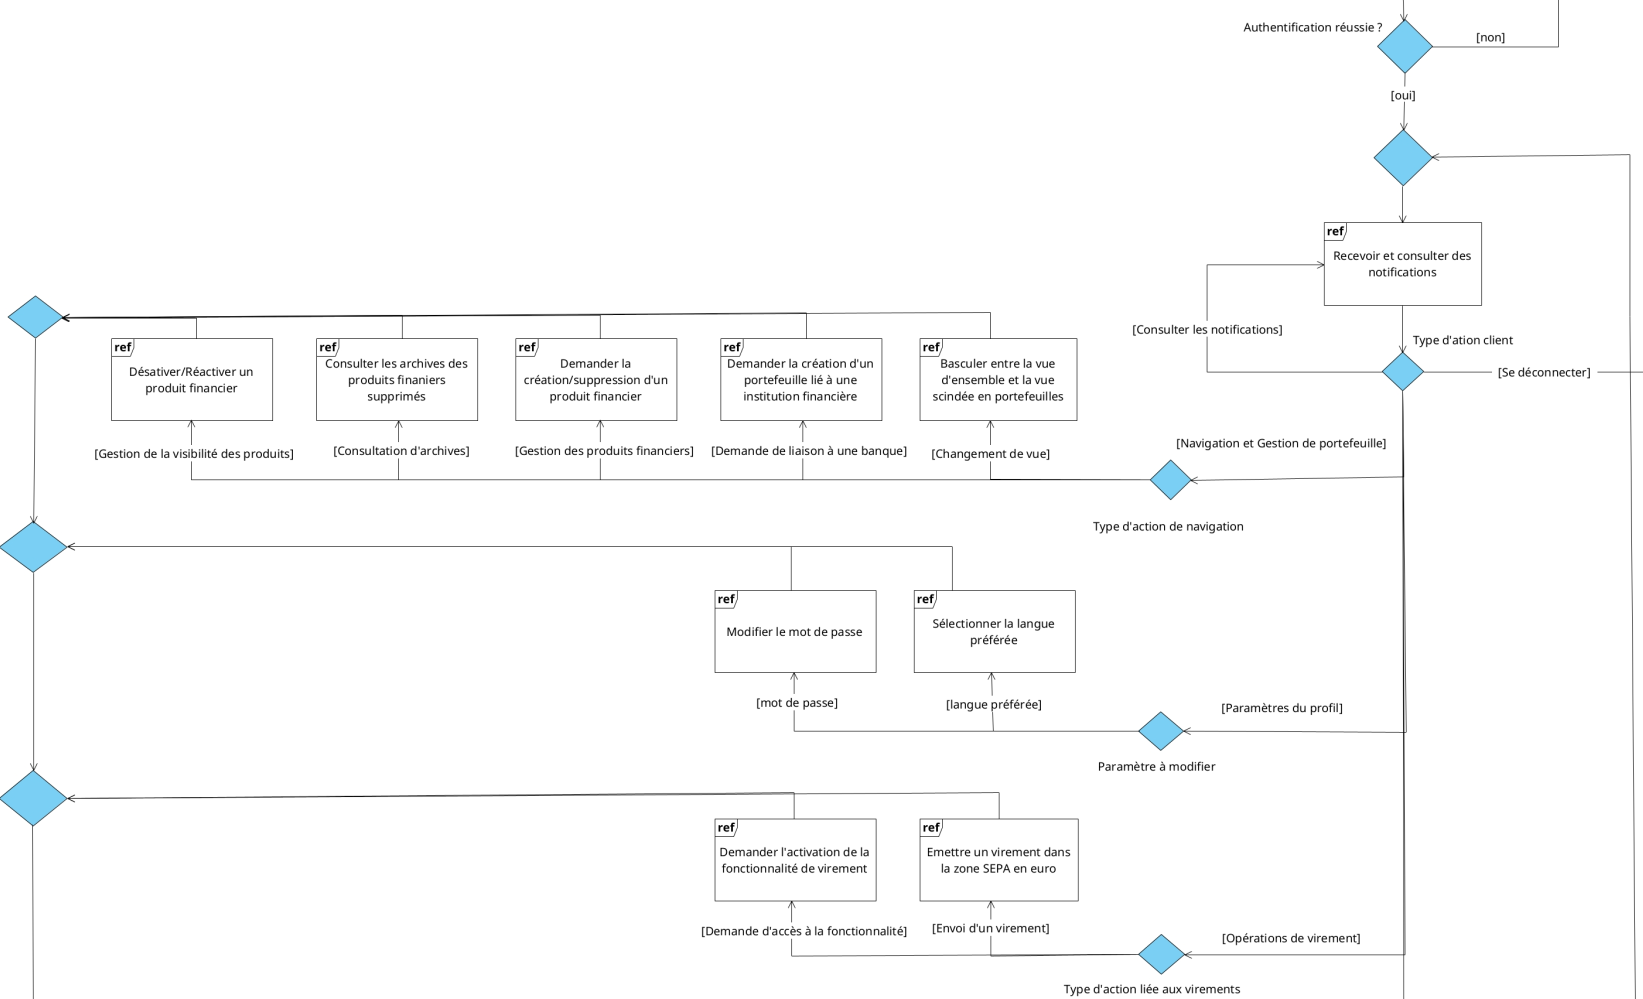
\includegraphics[width=1.0\textwidth]{IOD-Areas/ClientActionArea1.png}}
    \caption{Interaction Overview Diagram -- Actions client}
    \label{fig_iod_action_client}
\end{figure}

\begin{figure}[H]
    \centering
    \makebox[\textwidth][c]{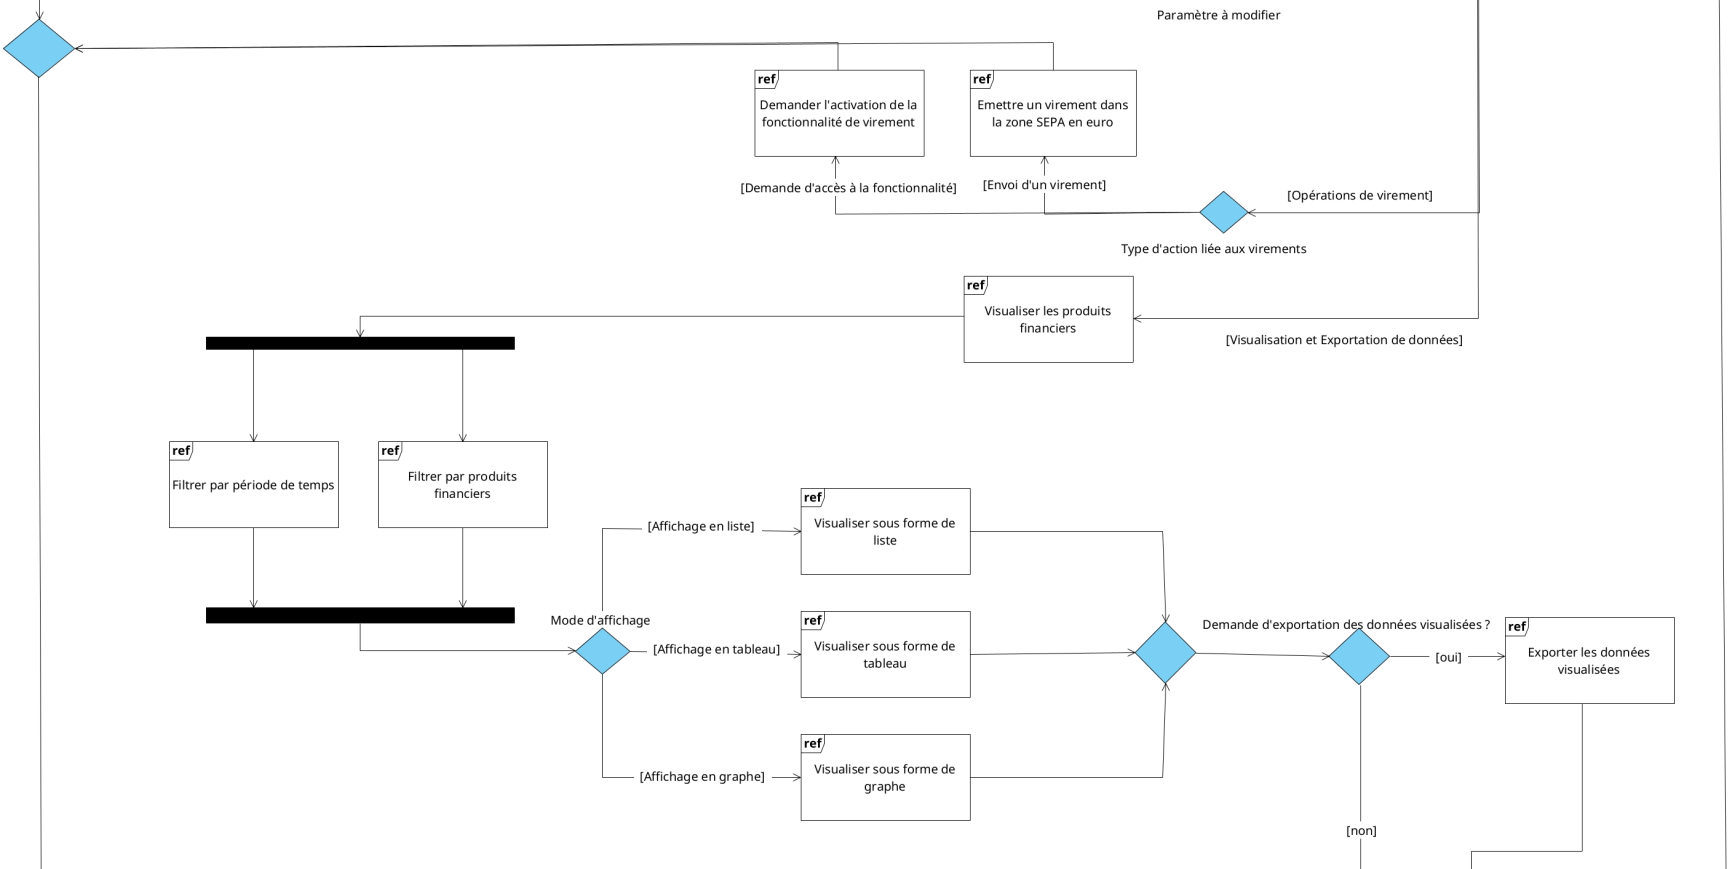
\includegraphics[width=1.0\textwidth]{IOD-Areas/ClientActionArea2.png}}
    \caption{Interaction Overview Diagram -- Visualisation et export de données}
    \label{fig_iod_visu_export}
\end{figure}

\subsubsection{IOD - Actions employé}
\begin{figure}[H]
    \centering
    \makebox[\textwidth][c]{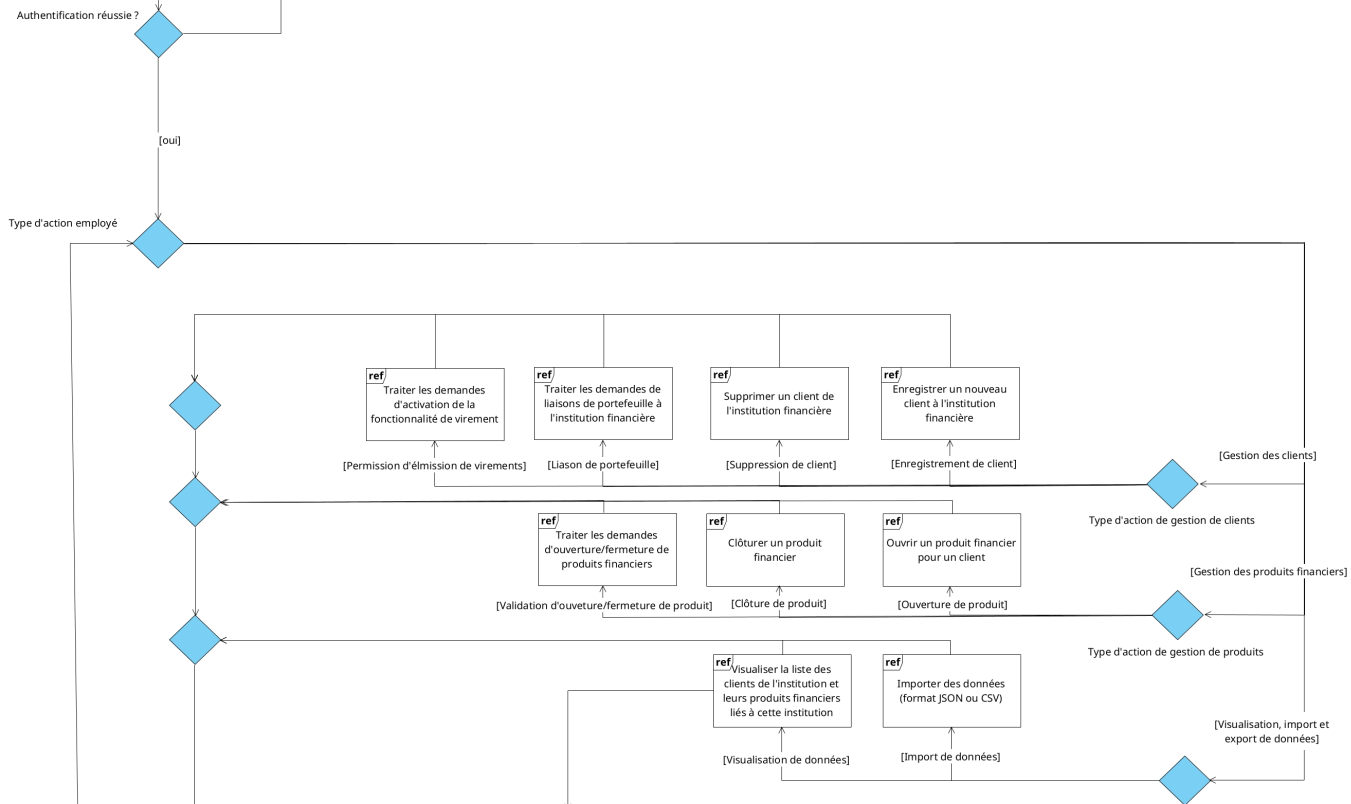
\includegraphics[width=0.9\textwidth]{IOD-Areas/EmpActionArea1.png}}
    \caption{Interaction Overview Diagram -- Actions employé}
    \label{fig_iod_action_emp}
\end{figure}

\begin{figure}[H]
    \centering
    \makebox[\textwidth][c]{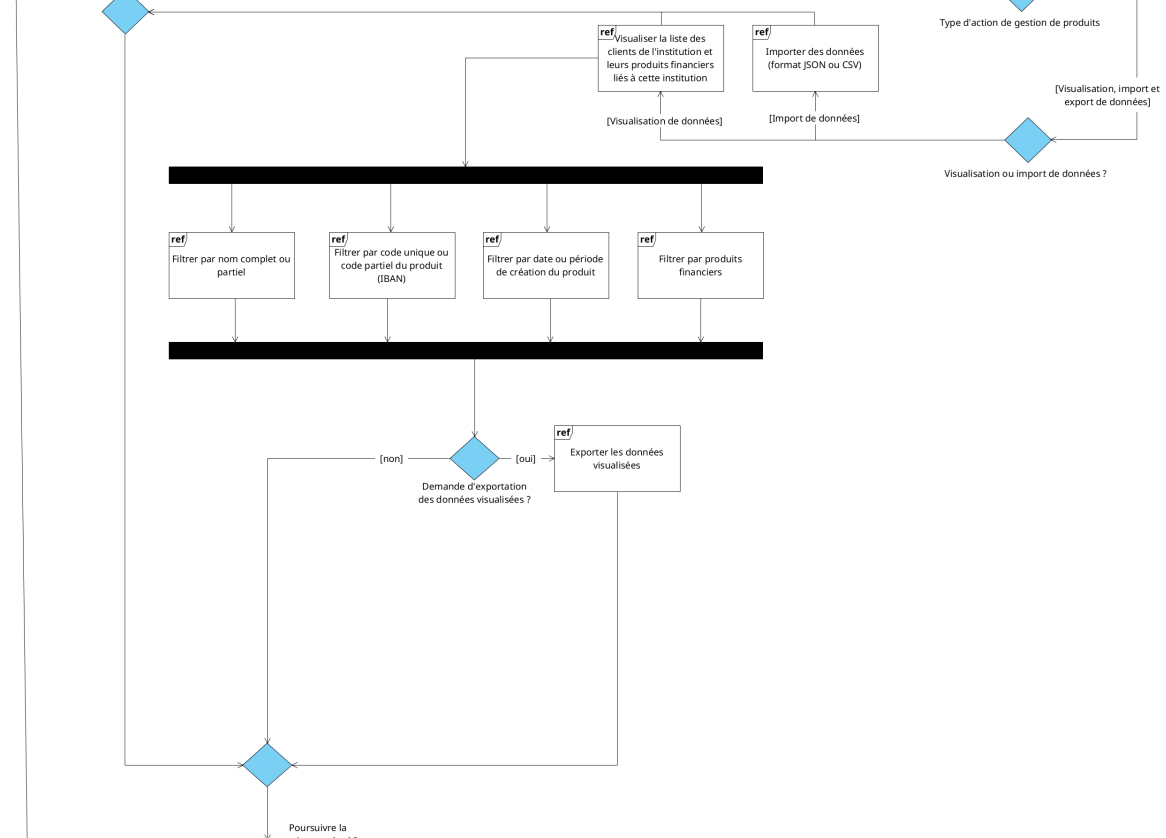
\includegraphics[width=0.9\textwidth]{IOD-Areas/EmpActionArea2.png}}
    \caption{Interaction Overview Diagram -- Visualisation, export et import de données}
    \label{fig_iod_visu_export_import_emp}
\end{figure}

\subsubsection{IOD - Phase de déconnexion}
\begin{figure}[H]
    \centering
    \makebox[\textwidth][c]{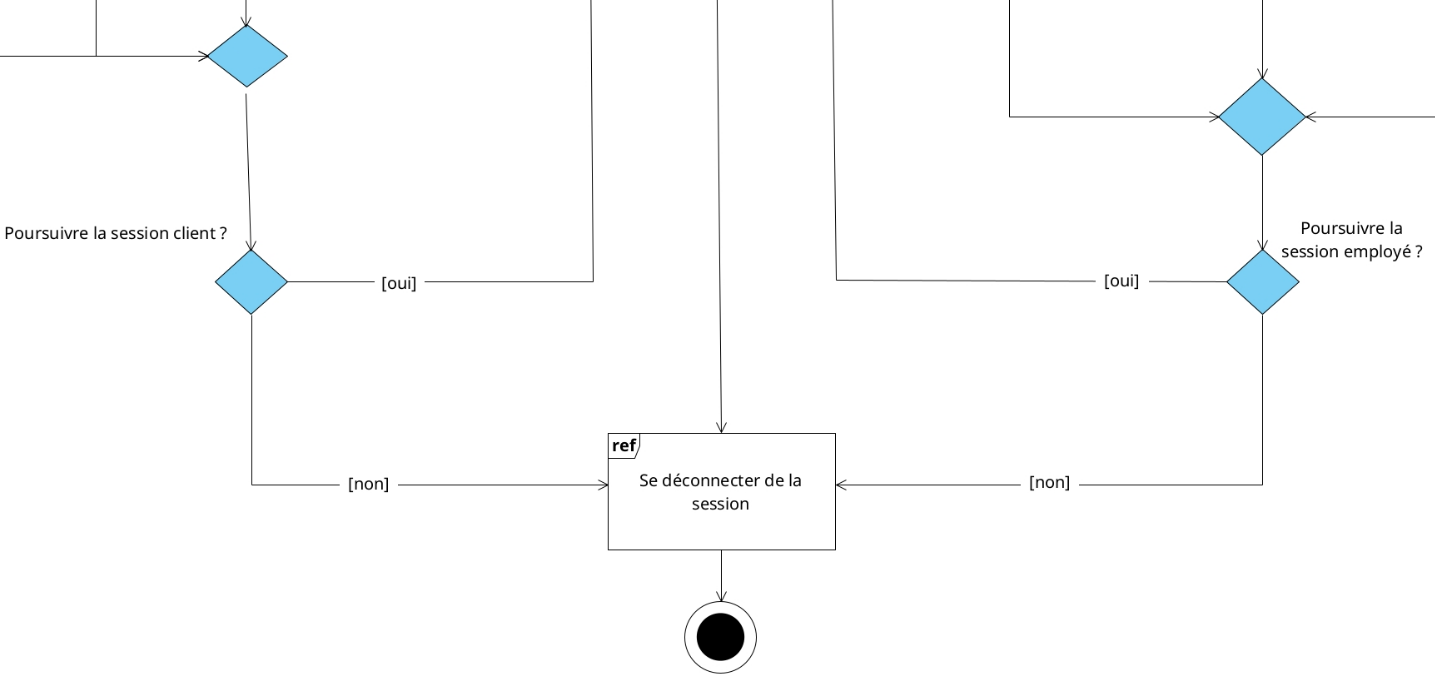
\includegraphics[width=1.0\textwidth]{IOD-Areas/DeconnexionArea.png}}
    \caption{Interaction Overview Diagram -- Phase de déconnexion}
    \label{fig_iod_déconnexion}
\end{figure}

\subsubsection{Explications de l'IOD}
Une fois la phase de connexion terminée, le diagramme se divise en deux parties : la connexion à l'espace client et à l'espace de gestion des clients de l'institution financières.
Le client ou l'employé de l'institution financière peuvent donc choisir d'effectuer n'importe quelle action dans leur espace de l'application. Une fois l'action effectuée, ils sont libres de poursuivre leur session, auquel cas ils retournent dans la séléction de leur prohaine action.
Dans le cas contraire, la phase de déconnexion débute et l'utilisateur (client ou employé) est déconnecté de sa session.
\vspace{0.3cm}
\\
\textit{NB : Les découpes du diagramme peuvent être consultées dans le sous-dossier IOD-Areas/ de l'archive contenant ce rapport.}
\pagebreak

\subsection{User Stories -- Fonctionnalités de base}
\textbf{UE :} S-INFO-015 Projet d'analyse et de conception logicielle\\
\textbf{Année académique :} 2026-2027\\
\textbf{Groupe :} G02 \textbf{Membres du groupe :} - Berkani Zinediné
(Matricule : 232034) - Fontaine Alexis (Matricule : 250602) - Quarta Hugo (Matricule
: 250711) - Vandooren Romain (Matricule : 251074)

\begin{center}\rule{0.5\linewidth}{0.5pt}\end{center}

\hypertarget{guxe9nuxe9ral}{%
\subsubsection{Général :}\label{guxe9nuxe9ral}}

\hypertarget{feature-internationalisation-et-gestion-des-langues}{%
\paragraph{1. Feature : Internationalisation et gestion des
langues}\label{feature-internationalisation-et-gestion-des-langues}}

\hypertarget{us1---support-multilingue}{%
\subparagraph{US1 - Support multilingue
:}\label{us1---support-multilingue}}

En tant que visiteur non-enregistré, je veux pouvoir choisir la langue
dans la page d'accueil afin de suivre les instructions d'enregistrement
dans cette langue.

\textbf{Critères d'acceptation :}

\begin{itemize}
\tightlist
\item
  La page d'accueil fournit un sélecteur de langue permettant de changer
  la langue d'affichage.
\item
  Toute information affichée utilise la langue sélectionnée.
\end{itemize}

\hypertarget{us2---choix-de-la-langue-pruxe9fuxe9ruxe9e-lors-de-la-cruxe9ation-dun-compte}{%
\subparagraph{US2 - Choix de la langue préférée lors de la création d'un
compte
:}\label{us2---choix-de-la-langue-pruxe9fuxe9ruxe9e-lors-de-la-cruxe9ation-dun-compte}}

En tant que visiteur non-enregistré, je veux indiquer et mémoriser ma
langue préférée afin d'utiliser l'application dans cette langue pour
toutes mes connections futures.

\textbf{Critères d'acceptation :}

\begin{itemize}
\tightlist
\item
  Le formulaire de création de compte propose un champ de choix de
  langue.
\item
  Ce champ obligatoire est pré-rempli avec une valeur par défaut qui
  peut être modifiée.
\item
  La langue choisie après validation du formulaire est enregistrée dans
  le profil utilisateur.
\end{itemize}

\hypertarget{us3---application-automatique-de-la-langue-pruxe9fuxe9ruxe9e-uxe0-chaque-connexion}{%
\subparagraph{US3 - Application automatique de la langue préférée à
chaque connexion
:}\label{us3---application-automatique-de-la-langue-pruxe9fuxe9ruxe9e-uxe0-chaque-connexion}}

En tant que titulaire, je veux que l'application utilise automatiquement
ma langue préférée afin de ne pas devoir la reconfigurer à chaque
session.

\textbf{Critères d'acceptation :}

\begin{itemize}
\tightlist
\item
  Après authentification, l'application utilise la langue enregistrée
  dans le profil utilisateur.
\item
  Ce comportement s'applique pendant toute la session.
\end{itemize}

\hypertarget{us4---modification-a-posteriori-de-la-langue-pruxe9fuxe9ruxe9e}{%
\subparagraph{US4 - Modification a posteriori de la langue préférée
:}\label{us4---modification-a-posteriori-de-la-langue-pruxe9fuxe9ruxe9e}}

En tant que titulaire, je veux pouvoir changer ma langue préférée afin
de utiliser l'application dans cette langue lors de la session actuelle
ainsi que toutes les sessions futures.

\textbf{Critères d'acceptation :}

\begin{itemize}
\tightlist
\item
  Une option dans le profil utilisateur permet de changer sa langue
  préférée.
\item
  Le changement se répercute immédiatement sur l'interface sans
  nécessiter une déconnexion et reconnexion.
\item
  La nouvelle préférence persiste lors des connexions suivantes.
\end{itemize}

\begin{center}\rule{0.5\linewidth}{0.5pt}\end{center}

\hypertarget{application-titulaire-pour-guxe9rer-ses-portefeuilles-financiers}{%
\subsubsection{Application titulaire pour gérer ses ``portefeuilles
financiers''
:}\label{application-titulaire-pour-guxe9rer-ses-portefeuilles-financiers}}

\hypertarget{feature-authentification-et-accuxe8s}{%
\paragraph{1. Feature : Authentification et
Accès}\label{feature-authentification-et-accuxe8s}}

\hypertarget{us5---inscription-dun-nouveau-titulaire}{%
\subparagraph{US5 - Inscription d'un nouveau
titulaire}\label{us5---inscription-dun-nouveau-titulaire}}

En tant que titulaire non-enregistré, je veux créer un compte
utilisateur en renseignant mon nom complet, mon numéro de registre
national, ma langue préférée et un mot de passe sécurisé afin de pouvoir
m'authentifier et gérer mes portefeuilles financiers.

\textbf{Critères d'acceptation :}

\begin{itemize}
\tightlist
\item
  Tous les champs du formulaire sont obligatoires : nom complet, numéro
  de registre national, langue préférée, mot de passe et confirmation du
  mot de passe.
\item
  Le numéro de registre national doit être valide.
\item
  Le mot de passe doit comporter au minimum 8 caractères, dont au moins
  une majuscule, un chiffre et un caractère spécial.
\item
  L'inscription est rejetée si un compte existe déjà avec le même numéro
  de registre national ou le même nom complet.
\item
  Le champ de langue préférée est pré-rempli avec la langue par défaut
  et peut être modifié.
\item
  Si tous les champs sont valides et que les mots de passe sont
  identiques, le compte est créé et l'utilisateur peut se connecter (ou
  est connecté automatiquement).
\end{itemize}

\hypertarget{us6---connexion-uxe0-lespace-titulaire}{%
\subparagraph{US6 - Connexion à l'espace
titulaire}\label{us6---connexion-uxe0-lespace-titulaire}}

En tant que titulaire, je veux me connecter à l'application avec mon nom
complet, mon numéro de registre national et mon mot de passe afin
d'accéder à mes portefeuilles financiers.

\textbf{Critères d'acceptation :}

\begin{itemize}
\tightlist
\item
  Le formulaire de connexion nécessite le nom complet, le numéro de
  registre national et le mot de passe.
\item
  Si les trois informations correspondent exactement à un compte
  enregistré, l'utilisateur est connecté et redirigé vers son tableau de
  bord.
\item
  Si au moins une information est incorrecte ou absente, l'accès est
  refusé avec un message d'erreur.
\item
  Un utilisateur ne peut avoir qu'une seule session active à la fois :
  la création d'une nouvelle session entraîne la fermeture de la
  précédente.
\item
  L'application permet à plusieurs utilisateurs différents d'être
  connectés simultanément.
\end{itemize}

\hypertarget{us7---ruxe9initialisation-dun-mot-de-passe-oubliuxe9}{%
\subparagraph{US7 - Réinitialisation d'un mot de passe
oublié}\label{us7---ruxe9initialisation-dun-mot-de-passe-oubliuxe9}}

En tant que titulaire ayant oublié son mot de passe,\\
je veux réinitialiser mon mot de passe depuis la page de connexion en
fournissant mes identifiants afin de recouvrer l'accès à mon espace
personnel.

\textbf{Critères d'acceptation :}

\begin{itemize}
\tightlist
\item
  Une option ``Mot de passe oublié'' est présente sur la page de
  connexion.
\item
  La réinitialisation du mot de passe nécessite le numéro de registre
  national et le nom complet associés au compte.
\item
  Si les informations fournies correspondent à un utilisateur
  enregistré, le formulaire permet de saisir un nouveau mot de passe et
  sa confirmation.
\item
  Le nouveau mot de passe doit respecter les mêmes règles de sécurité
  (minimum 8 caractères, majuscule, chiffre et caractère spécial).
\item
  Le nouveau mot de passe et la confirmation du nouveau mot de passe
  doivent être identiques pour valider la réinitialisation.
\item
  Si les données d'identification ne correspondent à aucun compte, la
  réinitialisation échoue avec un message d'erreur.
\item
  Une fois réinitialisé, l'ancien mot de passe est invalidé et
  l'utilisateur peut se connecter avec son nouveau mot de passe.
\end{itemize}

\hypertarget{us8---modification-du-mot-de-passe-depuis-le-profil}{%
\subparagraph{US8 - Modification du mot de passe depuis le
profil}\label{us8---modification-du-mot-de-passe-depuis-le-profil}}

En tant que titulaire,\\
je veux pouvoir modifier mon mot de passe actuel dans mes paramètres de
compte\\
afin de renforcer la sécurité de mon compte.

\textbf{Critères d'acceptation :}

\begin{itemize}
\tightlist
\item
  L'utilisateur doit saisir son mot de passe actuel, le nouveau mot de
  passe et la confirmation du nouveau mot de passe.
\item
  L'ancien mot de passe saisi doit être vérifié avant sa mise à jour.
\item
  Le nouveau mot de passe doit respecter les mêmes règles de sécurité et
  doit être différent du mot de passe actuel.
\item
  La mise à jour est immédiatement enregistrée.
\end{itemize}

\hypertarget{us9---duxe9connexion-de-lapplication}{%
\subparagraph{US9 - Déconnexion de
l'application}\label{us9---duxe9connexion-de-lapplication}}

En tant que titulaire connecté,\\
je veux pouvoir me déconnecter à tout moment de mon application afin de
terminer ma session.

\textbf{Critères d'acceptation :}

\begin{itemize}
\tightlist
\item
  Une option de déconnexion est accessible à tout instant.
\item
  La déconnexion termine la session et redirige vers la page de
  connexion.
\end{itemize}

\hypertarget{feature-gestion-des-portefeuilles-financiers}{%
\paragraph{2. Feature : Gestion des Portefeuilles
Financiers}\label{feature-gestion-des-portefeuilles-financiers}}

\hypertarget{us10---demande-de-cruxe9ation-et-liaison-dun-portefeuille-financier}{%
\subparagraph{US10 - Demande de création et liaison d'un portefeuille
financier}\label{us10---demande-de-cruxe9ation-et-liaison-dun-portefeuille-financier}}

En tant que titulaire, je veux soumettre une demande de création d'un
portefeuille lié à une institution financière afin d'accéder aux
produits financiers dont je suis titulaire.

\textbf{Critères d'acceptation :}

\begin{itemize}
\tightlist
\item
  L'utilisateur peut sélectionner une institution financière parmi la
  liste des banques enregistrées dans le système.
\item
  Une fois soumise, la demande apparaît avec le statut ``En attente de
  validation par l'institution''.
\item
  Si la demande est approuvée par l'institution financière :

  \begin{itemize}
  \tightlist
  \item
    Le portefeuille est automatiquement créé et devient accessible à
    l'utilisateur.
  \item
    Le portefeuille inclut au minimum le compte courant du titulaire.
  \item
    L'utilisateur a accès à tous les produits pour lesquels il est
    titulaire ou co-titulaire auprès de cette banque.
  \end{itemize}
\item
  Si la demande est refusée par l'institution financière :

  \begin{itemize}
  \tightlist
  \item
    L'utilisateur est informé par une notification du rejet de sa
    demande.
  \item
    Aucun portefeuille n'est créé pour cette institution.
  \end{itemize}
\end{itemize}

\hypertarget{us11---gestion-de-laffichage-des-produits}{%
\subparagraph{US11 - Gestion de l'affichage des
produits}\label{us11---gestion-de-laffichage-des-produits}}

En tant que titulaire, je veux désactiver ou réactiver certains produits
financiers de mon portefeuille afin de ne visualiser que les produits
que je souhaite gérer.

\textbf{Critères d'acceptation :}

\begin{itemize}
\tightlist
\item
  Seuls les produits activés par le client sont visibles dans son
  portefeuille.
\item
  Le client possède une option pour désactiver des produits de son
  portefeuille.
\item
  Le client a la possibilité de réactiver ses produits désactivés via
  une liste des produits masqués.
\end{itemize}

\hypertarget{us12---demande-douverture-ou-de-cluxf4ture-dun-produit-financier}{%
\subparagraph{US12 - Demande d'ouverture ou de clôture d'un produit
financier}\label{us12---demande-douverture-ou-de-cluxf4ture-dun-produit-financier}}

En tant que titulaire,\\
je veux introduire une demande d'ouverture ou de clôture d'un produit
financier auprès de mon institution financière afin de faire gérer la
création et la suppression de mes produits financiers directement depuis
l'application.

\textbf{Critères d'acceptation :}

\begin{itemize}
\tightlist
\item
  L'utilisateur peut soumettre une demande d'ouverture en choisissant le
  type de compte souhaité parmi les produits proposés par la banque du
  portefeuille.
\item
  L'utilisateur peut soumettre une demande de clôture pour un compte
  existant dont il est titulaire.
\item
  Une confirmation est demandée avant toute validation d'une demande de
  clôture.
\item
  Une fois envoyée, la demande apparaît sous le statut ``En attente de
  traitement par l'institution financière''.
\item
  Si la demande est approuvée par l'institution, le nouveau produit
  apparaît dans le portefeuille (ou le produit clôturé passe dans le
  statut archivé).
\item
  Si la demande est refusée par l'institution, le client reçoit une
  notification expliquant le rejet.
\end{itemize}

\hypertarget{us13---notifications-de-mise-uxe0-jour-du-portefeuille-et-consultation-des-archives}{%
\subparagraph{US13 - Notifications de mise à jour du portefeuille et
consultation des
archives}\label{us13---notifications-de-mise-uxe0-jour-du-portefeuille-et-consultation-des-archives}}

En tant que titulaire,\\
je veux être averti dès l'ouverture de mon portefeuille de tout ajout ou
suppression de produit effectué par ma banque afin de suivre l'état de
mes comptes.

\textbf{Critères d'acceptation :}

\begin{itemize}
\tightlist
\item
  À l'ouverture d'un portefeuille, si la banque a ajouté un ou plusieurs
  produits, une notification informe le titulaire et les produits sont
  automatiquement disponibles.
\item
  À l'ouverture d'un portefeuille, si la banque a supprimé un ou
  plusieurs produits, une notification est affichée au titulaire.
\end{itemize}

\hypertarget{us14---consultation-des-archives}{%
\subparagraph{US14 - Consultation des
archives}\label{us14---consultation-des-archives}}

En tant que titulaire, je veux accéder aux produits financiers archivés
afin de consulter l'historique des transactions de mes produits
financiers supprimés.

\textbf{Critères d'acceptation :}

\begin{itemize}
\tightlist
\item
  Tout produit financier clôturé passe automatiquement dans le statut
  ``archivé''.
\item
  Un produit archivé ne permet plus d'effectuer de nouvelles
  transactions financières.
\item
  L'utilisateur dispose d'une visualisation de l'historique complet des
  transactions de ses produits archivés.
\end{itemize}

\hypertarget{us15---bascule-entre-portefeuilles-et-vue-densemble}{%
\subparagraph{US15 - Bascule entre portefeuilles et vue
d'ensemble}\label{us15---bascule-entre-portefeuilles-et-vue-densemble}}

En tant que titulaire client de plusieurs institutions financières,\\
je veux pouvoir afficher la liste de tous mes portefeuilles et basculer
facilement d'un portefeuille à un autre afin de gérer individuellement
chacun de mes portefeuilles et avoir une vision d'ensemble de ceux-ci.

\textbf{Critères d'acceptation :}

\begin{itemize}
\tightlist
\item
  La page d'accueil de l'application affiche à l'utilisateur connecté la
  liste de ses portefeuilles financiers.
\item
  L'utilisateur peut cliquer sur un des portefeuilles de la liste afin
  de le consulter individuellement.
\item
  Une option ``Vue d'ensemble'' affiche l'ensemble des produits de tous
  les portefeuilles du client sur une même interface.
\end{itemize}

\hypertarget{feature-virements-bancaires}{%
\paragraph{3. Feature : Virements
Bancaires}\label{feature-virements-bancaires}}

\hypertarget{us16---demande-dactivation-de-la-fonctionnalituxe9-de-virement}{%
\subparagraph{US16 - Demande d'activation de la fonctionnalité de
virement}\label{us16---demande-dactivation-de-la-fonctionnalituxe9-de-virement}}

En tant que titulaire,\\
je veux soumettre une demande d'accès à la fonctionnalité de virement
auprès de mon institution financière afin d'obtenir l'autorisation de
transférer de l'argent depuis mes comptes liés à l'institution.

\textbf{Critères d'acceptation :}

\begin{itemize}
\tightlist
\item
  L'utilisateur peut soumettre une demande d'autorisation de virement
  pour son portefeuille.
\item
  Une fois soumise, la demande passe dans le statut ``En attente
  d'approbation par l'institution financière''.
\item
  Tant que la demande n'est pas approuvée, l'accès aux virements reste
  verrouillé sur ce portefeuille.
\item
  Si l'institution approuve la demande :

  \begin{itemize}
  \tightlist
  \item
    La permission est activée pour le titulaire.
  \item
    La fonctionnalité de virements devient accessible.
  \item
    L'utilisateur est informé de l'activation par une notification.
  \end{itemize}
\item
  Si l'institution refuse la demande :

  \begin{itemize}
  \tightlist
  \item
    L'utilisateur est notifié du rejet et la fonctionnalité reste
    verrouillée.
  \end{itemize}
\end{itemize}

\hypertarget{us17---uxe9mission-dun-virement-sepa-en-euros}{%
\subparagraph{US17 - Émission d'un virement SEPA en
euros}\label{us17---uxe9mission-dun-virement-sepa-en-euros}}

En tant que titulaire bénéficiant de l'autorisation de virement,\\
je veux effectuer un virement en euros vers un autre compte bancaire au
sein de la zone SEPA afin de transférer de l'argent vers mes propres
comptes ou un autre destinataire.

\textbf{Critères d'acceptation :}

\begin{itemize}
\tightlist
\item
  L'utilisateur sélectionne l'un de ses comptes comme compte source
  (émetteur).
\item
  Le formulaire nécessite la saisie du compte destinataire (IBAN
  valide), du montant (en euros avec au maximum 2 décimales) et du nom
  complet du destinataire.
\item
  L'utilisateur peut aussi ajouter :

  \begin{itemize}
  \tightlist
  \item
    Une communication libre ou structurée.
  \item
    Une date pour planifier l'exécution du virement à une date future.
  \end{itemize}
\item
  Si le nom saisi ne correspond pas exactement au nom du titulaire réel
  associé à l'IBAN destinataire, un avertissement est affiché à
  l'utilisateur avant la validation.
\item
  Si le destinataire ne se trouve pas dans la zone SEPA, l'opération est
  annulée avec un message d'erreur.
\item
  Si le solde du compte source n'est pas suffisant pour couvrir le
  montant du virement, celui-ci est annulé avec un message d'erreur.
\item
  L'opération nécessite une validation de sécurité obligatoire (saisie
  du mot de passe ou code de confirmation) avant l'exécution.
\item
  En cas de confirmation valide, le montant est débité du compte source,
  crédité sur le compte cible (ou programmé si date future) et une
  confirmation est affichée.
\end{itemize}

\hypertarget{feature-historique-visualisation-et-exportation}{%
\paragraph{4. Feature : Historique, Visualisation et
Exportation}\label{feature-historique-visualisation-et-exportation}}

\hypertarget{us18---consultation-et-filtrage-de-lhistorique-des-transactions}{%
\subparagraph{US18 - Consultation et filtrage de l'historique des
transactions}\label{us18---consultation-et-filtrage-de-lhistorique-des-transactions}}

En tant que titulaire,\\
je veux consulter l'historique des transactions pour un produit
spécifique ou pour un ensemble de produits sur une période définie afin
de vérifier mes opérations passées et visualiser l'évolution de mes
produits financiers.

\textbf{Critères d'acceptation :}

\begin{itemize}
\tightlist
\item
  L'utilisateur peut sélectionner un ou plusieurs comptes spécifiques au
  sein d'un portefeuille ou choisir l'ensemble de ses portefeuilles.
\item
  L'utilisateur peut définir la période de consultation des
  transactions.
\item
  La visualisation peut se faire sous forme de listes, de tableaux ou de
  graphes.
\item
  Chaque transaction affiche la date, le type d'opération, le montant
  (avec exactement 2 décimales), la devise et les informations du tiers
  (IBAN/nom).
\item
  Si aucune transaction n'existe sur la période sélectionnée, un message
  informatif est affiché.
\end{itemize}

\hypertarget{us19---exportation-des-donnuxe9es-historiques}{%
\subparagraph{US19 - Exportation des données
historiques}\label{us19---exportation-des-donnuxe9es-historiques}}

En tant que titulaire, je veux exporter les données de transactions
visualisées aux formats CSV et JSON,\\
afin de conserver une copie externe de mes relevés et pouvoir les
exploiter dans d'autres outils d'analyse.

\textbf{Critères d'acceptation :}

\begin{itemize}
\tightlist
\item
  L'interface propose des options de téléchargement aux formats CSV et
  JSON.
\item
  Le fichier exporté contient l'ensemble des transactions correspondant
  aux filtres actifs à l'écran (période et produits sélectionnés).
\item
  Le format des données exportées respecte la syntaxe standard (colonnes
  valides pour le CSV, structure d'objets valide pour le JSON).
\end{itemize}

\begin{center}\rule{0.5\linewidth}{0.5pt}\end{center}

\hypertarget{application-institution-financiuxe8re}{%
\subsubsection{Application Institution Financière
:}\label{application-institution-financiuxe8re}}

\hypertarget{feature-authentification-et-suxe9curituxe9-de-linstitution}{%
\paragraph{1. Feature : Authentification et Sécurité de
l'Institution}\label{feature-authentification-et-suxe9curituxe9-de-linstitution}}

\hypertarget{us20---connexion-de-linstitution-financiuxe8re}{%
\subparagraph{US20 - Connexion de l'institution
financière}\label{us20---connexion-de-linstitution-financiuxe8re}}

En tant qu'employé d'une institution financière,\\
je veux me connecter à l'application avec l'identifiant unique de mon
institution et son mot de passe\\
afin d'accéder à l'espace de gestion des clients et produits financiers
de ma banque.

\textbf{Critères d'acceptation :}

\begin{itemize}
\tightlist
\item
  Le formulaire nécessite la saisie de l'identifiant de l'institution
  (code SWIFT/BIC ou login institutionnel) et du mot de passe.
\item
  L'application utilise un accès unique pour l'ensemble des employés
  d'une même institution financière.
\item
  Si les identifiants correspondent, l'utilisateur est connecté et
  accède à l'espace de son institution.
\item
  Si l'identifiant ou le mot de passe est invalide, l'accès est refusé
  avec un message d'erreur.
\end{itemize}

\hypertarget{us21---modification-du-mot-de-passe-de-linstitution}{%
\subparagraph{US21 - Modification du mot de passe de
l'institution}\label{us21---modification-du-mot-de-passe-de-linstitution}}

En tant qu'employé connecté d'une institution financière,\\
je veux pouvoir modifier le mot de passe du compte de l'institution
depuis l'application\\
afin de renforcer la sécurité d'accès à ce compte.

\textbf{Critères d'acceptation :}

\begin{itemize}
\tightlist
\item
  Une option de changement de mot de passe est accessible depuis les
  paramètres de l'application.
\item
  La procédure nécessite la saisie de l'ancien mot de passe, du nouveau
  mot de passe et de la confirmation du nouveau mot de passe.
\item
  L'ancien mot de passe doit être validé avant sa modification.
\item
  Le nouveau mot de passe doit respecter les mêmes règles de sécurité et
  être différent de l'actuel.
\item
  Une fois modifié, le nouveau mot de passe est immédiatement actif pour
  toutes les prochaines connexions de l'institution.
\end{itemize}

\hypertarget{us22---duxe9connexion-de-lespace-institutionnel}{%
\subparagraph{US22 - Déconnexion de l'espace
institutionnel}\label{us22---duxe9connexion-de-lespace-institutionnel}}

En tant qu'employé connecté d'une institution financière,\\
je veux pouvoir me déconnecter à tout moment de l'application,\\
afin de fermer la session administrative.

\textbf{Critères d'acceptation :}

\begin{itemize}
\tightlist
\item
  Une option de déconnexion est accessible à tout instant.
\item
  La déconnexion met immédiatement fin à la session en cours et redirige
  vers la page de connexion.
\end{itemize}

\hypertarget{feature-gestion-des-clients-et-des-produits-financiers}{%
\paragraph{2. Feature : Gestion des Clients et des Produits
Financiers}\label{feature-gestion-des-clients-et-des-produits-financiers}}

\hypertarget{us23---enregistrement-dun-nouveau-client-aupruxe8s-de-linstitution}{%
\subparagraph{US23 - Enregistrement d'un nouveau client auprès de
l'institution}\label{us23---enregistrement-dun-nouveau-client-aupruxe8s-de-linstitution}}

En tant qu'employé connecté d'une institution financière,\\
je veux enregistrer un client en renseignant son identité,\\
afin de lui permettre de souscrire à nos produits financiers.

\textbf{Critères d'acceptation :}

\begin{itemize}
\tightlist
\item
  L'enregistrement nécessite la saisie du nom complet et du numéro de
  registre national.
\item
  L'opération est refusée si le client est déjà enregistré auprès de
  notre institution financière.
\item
  Une fois enregistré, le client apparaît immédiatement dans la liste
  des clients de l'institution.
\item
  L'employé n'a accès qu'à la liste des clients enregistrés auprès de sa
  propre institution.
\end{itemize}

\hypertarget{us24---suppression-dun-client-de-linstitution}{%
\subparagraph{US24 - Suppression d'un client de
l'institution}\label{us24---suppression-dun-client-de-linstitution}}

En tant qu'employé connecté d'une institution financière,\\
je veux supprimer un client de notre institution,\\
afin de mettre fin à son contrat avec notre institution.

\textbf{Critères d'acceptation :}

\begin{itemize}
\tightlist
\item
  L'employé peut sélectionner un client lié à son institution et
  demander sa suppression.
\item
  Le client supprimé n'apparaît plus dans la liste des clients de
  l'institution.
\end{itemize}

\hypertarget{us25---ouverture-dun-produit-financier-pour-un-client}{%
\subparagraph{US25 - Ouverture d'un produit financier pour un
client}\label{us25---ouverture-dun-produit-financier-pour-un-client}}

En tant qu'employé connecté d'une institution financière,\\
je veux ouvrir un nouveau produit financier pour l'un de nos clients,\\
afin de lui fournir un nouveau compte répondant à ses besoins bancaires.

\textbf{Critères d'acceptation :}

\begin{itemize}
\tightlist
\item
  L'employé sélectionne un client existant de l'institution et choisit
  un type de compte à ouvrir (compte courant, compte jeune, compte
  épargne, compte à terme,\ldots).
\item
  Le système génère automatiquement un identifiant unique (code IBAN
  conforme) associé au code BIC/SWIFT de l'institution.
\item
  Le produit créé apparaît dans la liste des produits financiers gérés
  par l'institution.
\item
  L'employé n'a accès à la gestion qu'aux produits fournis par sa propre
  institution.
\end{itemize}

\hypertarget{us26---cluxf4ture-dun-produit-financier}{%
\subparagraph{US26 - Clôture d'un produit
financier}\label{us26---cluxf4ture-dun-produit-financier}}

En tant qu'employé connecté d'une institution financière,\\
je veux clôturer un produit financier détenu par un client auprès de
notre institution,\\
afin de résilier ce contrat bancaire.

\textbf{Critères d'acceptation :}

\begin{itemize}
\tightlist
\item
  L'employé peut clôturer un produit actif de son institution pour un de
  ses clients à condition que celui-ci ait un solde nul.
\item
  Si le solde du produit financier n'est pas nul, l'opération est
  annulée et un message d'erreur est affiché.
\item
  Dès la suppression, le produit passe dans le statut ``archivé''.
\item
  L'historique des opérations passées du produit archivé reste conservé.
\end{itemize}

\hypertarget{feature-traitement-des-demandes-clients}{%
\paragraph{3. Feature : Traitement des demandes
clients}\label{feature-traitement-des-demandes-clients}}

\hypertarget{us27---traitement-des-demandes-douverture-et-de-cluxf4ture-de-produits-financiers}{%
\subparagraph{US27 - Traitement des demandes d'ouverture et de clôture
de produits
financiers}\label{us27---traitement-des-demandes-douverture-et-de-cluxf4ture-de-produits-financiers}}

En tant qu'employé connecté d'une institution financière, je veux
consulter, approuver ou refuser les demandes d'ouverture et de clôture
de comptes formulées par nos clients afin de gérer l'ensemble de leurs
produits financiers liés à notre institution.

\textbf{Critères d'acceptation :}

\begin{itemize}
\tightlist
\item
  L'employé peut consulter l'ensemble des demandes d'ouverture et de
  clôture de produits en attente pour les clients de son institution.
\item
  Pour une demande d'ouverture :

  \begin{itemize}
  \tightlist
  \item
    Si la demande est approuvée, le produit est créé avec un code IBAN
    conforme, est lié au client passe dans l'état actif et une
    notification de succès est envoyée au client.
  \item
    Si la demande est refusée, le client reçoit une notification
    expliquant le refus et la demande est clôturée.
  \end{itemize}
\item
  Pour une demande de clôture :

  \begin{itemize}
  \tightlist
  \item
    Si la demande est approuvée, le produit est supprimé, passe dans
    l'état archivé et une notification de succès est envoyée au client.
  \item
    Si la demande est refusée, le client reçoit une notification
    expliquant le refus et la demande est clôturée.
  \end{itemize}
\end{itemize}

\hypertarget{us28---traitement-des-demandes-de-liaison-de-portefeuille}{%
\subparagraph{US28 - Traitement des demandes de liaison de
portefeuille}\label{us28---traitement-des-demandes-de-liaison-de-portefeuille}}

En tant qu'employé connecté d'une institution financière, je veux
consulter, approuver ou refuser les demandes de liaisons de portefeuille
émises par nos clients afin de contrôler l'accès de nos clients à nos
produits.

\textbf{Critères d'acceptation :}

\begin{itemize}
\tightlist
\item
  L'employé peut consulter les demandes de liaisons de portefeuille en
  attente des clients de son institution.
\item
  Si la demande est approuvée, tous les produits du client liés à
  l'institution lui sont rendus visibles.
\item
  Si la demande est refusée, le client reçoit une notification
  expliquant le refus et la demande est clôturée.
\end{itemize}

\hypertarget{us29---traitement-des-demandes-dactivation-des-virements}{%
\subparagraph{US29 - Traitement des demandes d'activation des
virements}\label{us29---traitement-des-demandes-dactivation-des-virements}}

En tant qu'employé connecté d'une institution financière, je veux
consulter, approuver ou refuser les demandes d'autorisation de virement
émises par nos clients afin de contrôler l'accès de nos clients à cette
fonctionnalité.

\textbf{Critères d'acceptation :}

\begin{itemize}
\tightlist
\item
  L'employé peut consulter les demandes d'autorisation de virement en
  attente des clients de son institution.
\item
  Si la demande est approuvée, la permission de virement est débloquée
  pour le client et celui-ci en est notifié.
\item
  Si la demande est refusée, la fonctionnalité de virement reste
  verrouillée pour ce client et celui-ci est averti du refus par une
  notification.
\end{itemize}

\hypertarget{feature-visualisation-filtrage-export-et-import}{%
\paragraph{4. Feature : Visualisation, filtrage, export et
import}\label{feature-visualisation-filtrage-export-et-import}}

\hypertarget{us30---consultation-et-filtrage-des-clients-et-des-produits}{%
\subparagraph{US30 - Consultation et filtrage des clients et des
produits}\label{us30---consultation-et-filtrage-des-clients-et-des-produits}}

En tant qu'employé connecté d'une institution financière,\\
je veux lister et filtrer l'ensemble des clients et produits financiers
de mon institution,\\
afin d'accéder rapidement aux informations de nos comptes.

\textbf{Critères d'acceptation :}

\begin{itemize}
\tightlist
\item
  L'employé peut consulter l'entièreté des clients liés à son
  institution et des produits financiers associés.
\item
  L'interface fournit des outils de recherche et de filtrage permettant
  de combiner :

  \begin{itemize}
  \tightlist
  \item
    La recherche par nom complet ou nom partiel du client.
  \item
    Le filtrage par type de produit financier (compte courant, épargne,
    terme,\ldots).
  \item
    La recherche par code unique ou code partiel du produit (IBAN).
  \item
    Le filtrage par date ou période de création du produit financier.
  \end{itemize}
\item
  Les données affichées se mettent à jour dynamiquement selon les
  filtres appliqués.
\item
  L'employé ne peut consulter aucun produit lié à une autre institution.
\end{itemize}

\hypertarget{us31---exportation-des-donnuxe9es-clients-et-produits-de-linstitution}{%
\subparagraph{US31 - Exportation des données clients et produits de
l'institution}\label{us31---exportation-des-donnuxe9es-clients-et-produits-de-linstitution}}

En tant qu'employé connecté d'une institution financière,\\
je veux exporter la liste filtrée des clients et des produits de notre
institution aux formats CSV et JSON,\\
afin de conserver nos données en dehors de l'application.

\textbf{Critères d'acceptation :}

\begin{itemize}
\tightlist
\item
  L'interface propose des options de téléchargement aux formats standard
  CSV et JSON.
\item
  Le fichier exporté contient exactement les données correspondant aux
  filtres sélectionnés.
\end{itemize}

\hypertarget{us32---importation-de-donnuxe9es-et-peuplement-de-la-base-de-donnuxe9es}{%
\subparagraph{US32 - Importation de données et peuplement de la base de
données}\label{us32---importation-de-donnuxe9es-et-peuplement-de-la-base-de-donnuxe9es}}

En tant qu'employé connecté d'une institution financière,\\
je veux importer un fichier de données (CSV ou JSON) dans
l'application,\\
afin d'initialiser ou de mettre à jour la base de données de notre
institution sans devoir le faire à la main.

\textbf{Critères d'acceptation :}

\begin{itemize}
\tightlist
\item
  L'employé peut charger un fichier de données au format CSV ou JSON.
\item
  Si le fichier contient des données liées à une autre institution
  financière, l'importation est rejetée avec un message d'erreur.
\item
  Si le fichier est valide, les données sont enregistrées et la liste
  des clients/produits est immédiatement mise à jour dans l'application.
\end{itemize}


\section{Extensions individuelles}

\subsection{Extension 1 : Paiement et gestion de fraudes -- Berkani Zinediné}
\subsubsection{Diagramme de cas d'utilisation}
\begin{figure}[H]
    \centering
    % \includegraphics[width=0.8\textwidth]{images/uc_extension1.png}
    \caption{Cas d'utilisation -- Extension 1}
\end{figure}
\subsubsection{Interaction Overview Diagram}
\begin{figure}[H]
    \centering
    % \includegraphics[width=0.8\textwidth]{images/iod_extension1.png}
    \caption{Interaction Overview Diagram -- Extension 1}
\end{figure}
\subsubsection{User Stories}
% \input{extension1-user-stories.tex}

\subsection{Extension 2 : Gestion de cartes -- Fontaine Alexis}
\subsubsection{Diagramme de cas d'utilisation}
\begin{figure}[H]
    \centering
    % \includegraphics[width=0.8\textwidth]{images/uc_extension2.png}
    \caption{Cas d'utilisation -- Extension 2}
\end{figure}
\subsubsection{Interaction Overview Diagram}
\begin{figure}[H]
    \centering
    % \includegraphics[width=0.8\textwidth]{images/iod_extension2.png}
    \caption{Interaction Overview Diagram -- Extension 2}
\end{figure}
\subsubsection{User Stories}
% \input{extension2-user-stories.tex}

\subsection{Extension 3 : Gestion du budget financier -- Quarta Hugo}
\subsubsection{Diagramme de cas d'utilisation}
\begin{figure}[H]
    \centering
    % \includegraphics[width=0.8\textwidth]{images/uc_extension3.png}
    \caption{Cas d'utilisation -- Extension 3}
    \label{fig_uc_ext3}
\end{figure}
\subsubsection{Interaction Overview Diagram}
\begin{figure}[H]
    \centering
    % \includegraphics[width=0.8\textwidth]{images/iod_extension3.png}
    \caption{Interaction Overview Diagram -- Extension 3}
    \label{fig_iod_ext3}
\end{figure}
\subsubsection{User Stories}
% \input{extension3-user-stories.tex}

\subsection{Extension 4 : Gestion des placements -- Vandooren Romain}
\subsubsection{Diagramme de cas d'utilisation}
\begin{figure}[H]
    \centering
    % \includegraphics[width=0.8\textwidth]{images/uc_extension4.png}
    \caption{Cas d'utilisation -- Extension 4}
\end{figure}
\subsubsection{Interaction Overview Diagram}
\begin{figure}[H]
    \centering
    % \includegraphics[width=0.8\textwidth]{images/iod_extension4.png}
    \caption{Interaction Overview Diagram -- Extension 4}
\end{figure}
\subsubsection{User Stories}
% \input{extension4-user-stories.tex}

\end{document}